\chapter{ならし解析 - Amortized analysis}

\index{amortized analysis}

多くのプログラムにおいて、時間計算量は、アルゴリズムの構造を調べるだけで簡単に解析できます。
これは、どんなループを含み、何回ループが実行されるかといった解析を行います。
ただし、直感的な解析だけでは、計算量を正しく見積もれないこともあります。

\key{ならし解析 - Amortized analysis} を使って、時間計算量が一定に定まらないような計算量を見積もることができます。
基本的なアイデアは、個々の操作に注目するのではなく、アルゴリズムの実行中に全ての操作に使用される操作の合計時間を推定することです。

\section{2ポインタ - Two pointers method}

\index{two pointers method}

\key{2ポインタテクニック - two pointers method}
では、決められた方向にしか動かない2つのポインタを用いて処理を行います。
これにより、アルゴリズムの最大の動作時間が保証されます。
この例を2つ見ていきましょう。

\subsubsection{連続部分配列の和 - Subarray sum}

まず、$n$個の正の整数からなる配列と$x$が与えられたとき、
和が$x$となる連続した部分配列を見つけるか、
そのような部分配列はないと出力する問題を考えます。

例えば配列は以下のように与えられます。
\begin{center}
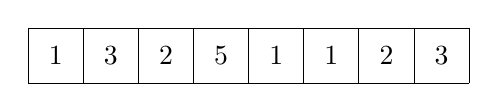
\begin{tikzpicture}[scale=0.7]
\draw (0,0) grid (8,1);

\node at (0.5,0.5) {$1$};
\node at (1.5,0.5) {$3$};
\node at (2.5,0.5) {$2$};
\node at (3.5,0.5) {$5$};
\node at (4.5,0.5) {$1$};
\node at (5.5,0.5) {$1$};
\node at (6.5,0.5) {$2$};
\node at (7.5,0.5) {$3$};
\end{tikzpicture}
\end{center}
これは、和が$8$となる連続部分配列があります。
\begin{center}
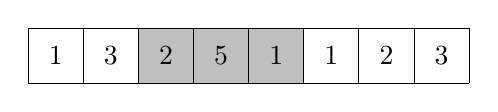
\begin{tikzpicture}[scale=0.7]
\fill[color=lightgray] (2,0) rectangle (5,1);
\draw (0,0) grid (8,1);

\node at (0.5,0.5) {$1$};
\node at (1.5,0.5) {$3$};
\node at (2.5,0.5) {$2$};
\node at (3.5,0.5) {$5$};
\node at (4.5,0.5) {$1$};
\node at (5.5,0.5) {$1$};
\node at (6.5,0.5) {$2$};
\node at (7.5,0.5) {$3$};
\end{tikzpicture}
\end{center}

この問題は、2ポインターを使うことで$O(n)$時間で解くことができます。
これは、部分配列の最初と最後の場所を指すポインタを保持し、
各ステップでにおいて、右ポインタを右にシフトしても和が$x$以下であるなら、ポインタを右にシフトします。
そうでなければ左ポインタを左にシフトします。
そして。和がちょうど$x$になれば、 解が見つかったことになります。


ここで、$x=8$を達成するための例を見てみましょう。
\begin{center}
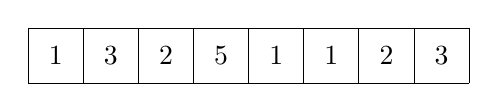
\begin{tikzpicture}[scale=0.7]
\draw (0,0) grid (8,1);

\node at (0.5,0.5) {$1$};
\node at (1.5,0.5) {$3$};
\node at (2.5,0.5) {$2$};
\node at (3.5,0.5) {$5$};
\node at (4.5,0.5) {$1$};
\node at (5.5,0.5) {$1$};
\node at (6.5,0.5) {$2$};
\node at (7.5,0.5) {$3$};
\end{tikzpicture}
\end{center}

まず、いくつか右ポインタを進め、
1, 3, 2 まで進めると和は6です。

\begin{center}
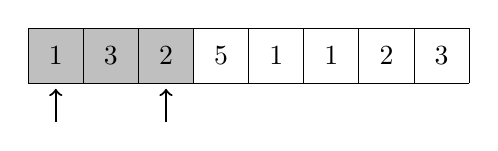
\begin{tikzpicture}[scale=0.7]
\fill[color=lightgray] (0,0) rectangle (3,1);
\draw (0,0) grid (8,1);

\node at (0.5,0.5) {$1$};
\node at (1.5,0.5) {$3$};
\node at (2.5,0.5) {$2$};
\node at (3.5,0.5) {$5$};
\node at (4.5,0.5) {$1$};
\node at (5.5,0.5) {$1$};
\node at (6.5,0.5) {$2$};
\node at (7.5,0.5) {$3$};

\draw[thick,->] (0.5,-0.7) -- (0.5,-0.1);
\draw[thick,->] (2.5,-0.7) -- (2.5,-0.1);
\end{tikzpicture}
\end{center}

ここで、右のポインタを進めると$x$を超えてしまうので、
左のポインタを右に動かすことにします。

\begin{center}
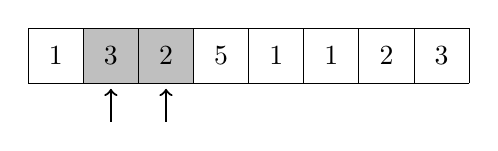
\begin{tikzpicture}[scale=0.7]
\fill[color=lightgray] (1,0) rectangle (3,1);
\draw (0,0) grid (8,1);

\node at (0.5,0.5) {$1$};
\node at (1.5,0.5) {$3$};
\node at (2.5,0.5) {$2$};
\node at (3.5,0.5) {$5$};
\node at (4.5,0.5) {$1$};
\node at (5.5,0.5) {$1$};
\node at (6.5,0.5) {$2$};
\node at (7.5,0.5) {$3$};

\draw[thick,->] (1.5,-0.7) -- (1.5,-0.1);
\draw[thick,->] (2.5,-0.7) -- (2.5,-0.1);
\end{tikzpicture}
\end{center}

ただし、この状態でも5を加えると$x$を超えてしまうので、左のポインタを右に進めます。
こうすると右のポインタを右に進められることになり、$2+5+1=8$となって$x$を見つけることができました。

\begin{center}
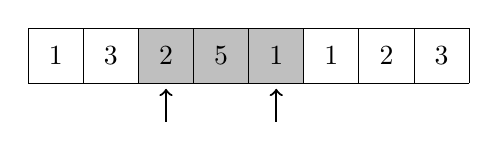
\begin{tikzpicture}[scale=0.7]
\fill[color=lightgray] (2,0) rectangle (5,1);
\draw (0,0) grid (8,1);

\node at (0.5,0.5) {$1$};
\node at (1.5,0.5) {$3$};
\node at (2.5,0.5) {$2$};
\node at (3.5,0.5) {$5$};
\node at (4.5,0.5) {$1$};
\node at (5.5,0.5) {$1$};
\node at (6.5,0.5) {$2$};
\node at (7.5,0.5) {$3$};

\draw[thick,->] (2.5,-0.7) -- (2.5,-0.1);
\draw[thick,->] (4.5,-0.7) -- (4.5,-0.1);
\end{tikzpicture}
\end{center}

このアルゴリズムの実行時間は、まず、右ポインタの移動ステップ数に注目します。
ポインタが1回のターンで何ステップ動けるかというのは配列によって異なります。
ただし、ポインタは右にしか動かないので、アルゴリズム中に合計$O(n)$ステップです。
ここで、左のポインタはアルゴリズム中に$O(n)$ステップ移動するので、このアルゴリズムは$O(n)$で動作する。

\subsubsection{2SUM problem}

\index{2SUM問題 - 2SUM problem}

他の問題を考えます。$n$個の数値からなる配列と$x$が与えられたとき、
和が$x$となる配列の2つの要素見つけるか、そのような値は存在しないことを出力しなさい、という問題です。
まず、配列の値を昇順に並べ替えます。
次に、2つのポインタを用いて配列を繰り返し処理します。
左のポインタは最初の値から始まり、1ターンごとに1ステップ右へ移動させます。
右のポインタは最後の値から始まり、左と右の値の合計が最大で$x$になるまで常に左に移動します。
例えば、次のような配列で、対象の和が$x=12$である場合を考える。

\begin{center}
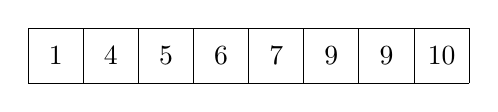
\begin{tikzpicture}[scale=0.7]
\draw (0,0) grid (8,1);

\node at (0.5,0.5) {$1$};
\node at (1.5,0.5) {$4$};
\node at (2.5,0.5) {$5$};
\node at (3.5,0.5) {$6$};
\node at (4.5,0.5) {$7$};
\node at (5.5,0.5) {$9$};
\node at (6.5,0.5) {$9$};
\node at (7.5,0.5) {$10$};
\end{tikzpicture}
\end{center}

ポインタの初期位置は以下の通りです。値の和は$1+10=11$で$x$より小さいです。

\begin{center}
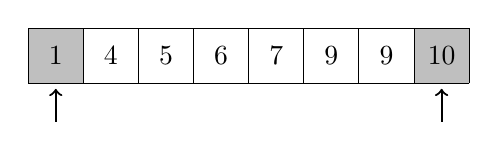
\begin{tikzpicture}[scale=0.7]
\fill[color=lightgray] (0,0) rectangle (1,1);
\fill[color=lightgray] (7,0) rectangle (8,1);
\draw (0,0) grid (8,1);

\node at (0.5,0.5) {$1$};
\node at (1.5,0.5) {$4$};
\node at (2.5,0.5) {$5$};
\node at (3.5,0.5) {$6$};
\node at (4.5,0.5) {$7$};
\node at (5.5,0.5) {$9$};
\node at (6.5,0.5) {$9$};
\node at (7.5,0.5) {$10$};

\draw[thick,->] (0.5,-0.7) -- (0.5,-0.1);
\draw[thick,->] (7.5,-0.7) -- (7.5,-0.1);
\end{tikzpicture}
\end{center}

そこで、左のポインタが右に1ステップ移動します。
ここで、右のポインターは左に3ステップ移動し、合計は$4 + 7 = 11$となる。

\begin{center}
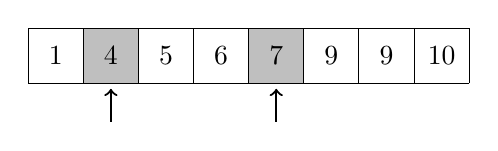
\begin{tikzpicture}[scale=0.7]
\fill[color=lightgray] (1,0) rectangle (2,1);
\fill[color=lightgray] (4,0) rectangle (5,1);
\draw (0,0) grid (8,1);

\node at (0.5,0.5) {$1$};
\node at (1.5,0.5) {$4$};
\node at (2.5,0.5) {$5$};
\node at (3.5,0.5) {$6$};
\node at (4.5,0.5) {$7$};
\node at (5.5,0.5) {$9$};
\node at (6.5,0.5) {$9$};
\node at (7.5,0.5) {$10$};

\draw[thick,->] (1.5,-0.7) -- (1.5,-0.1);
\draw[thick,->] (4.5,-0.7) -- (4.5,-0.1);
\end{tikzpicture}
\end{center}


ここで、左ポインタは再び右へ1ステップ移動します。
右のポインタは動かないため、$5+7=12$という解が存在することが分かりました。

\begin{center}
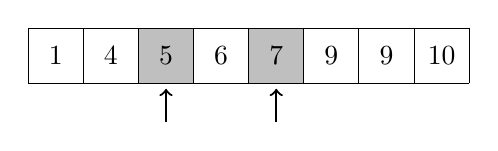
\begin{tikzpicture}[scale=0.7]
\fill[color=lightgray] (2,0) rectangle (3,1);
\fill[color=lightgray] (4,0) rectangle (5,1);
\draw (0,0) grid (8,1);

\node at (0.5,0.5) {$1$};
\node at (1.5,0.5) {$4$};
\node at (2.5,0.5) {$5$};
\node at (3.5,0.5) {$6$};
\node at (4.5,0.5) {$7$};
\node at (5.5,0.5) {$9$};
\node at (6.5,0.5) {$9$};
\node at (7.5,0.5) {$10$};

\draw[thick,->] (2.5,-0.7) -- (2.5,-0.1);
\draw[thick,->] (4.5,-0.7) -- (4.5,-0.1);
\end{tikzpicture}
\end{center}

実行時間は、
まず配列を$O(n \log n)$でソートし、次に両方のポインタを$O(n)$回移動させるため、$O(n \log n)$となります。
なお、二分探索を用いれば、別の方法で$O(n \log n)$時間で解くこともできます。
これは、配列を繰り返し、配列の各値に対して、和xをもたらす別の値を二分探索を行うことで行います。

\index{3SUM problem}
これより難しい問題としては、和が$x$となる3つの配列値を求める\key{3SUM 問題} があります。
上記のアルゴリズムの考え方を用いると,この問題は に従って O(n2 ) 時間で解くことができます。
\footnote{長い間、3SUM 問題を $O(n^2)$ 時間より効率的に解くことは不可能と考えられていました。し
かし、2014 年に、そうではないことが判明した \cite{gro14} }.

\section{Nearest smaller elements}

\index{nearest smaller elements}

Amortized analysis is often used to
estimate the number of operations
performed on a data structure.
The operations may be distributed unevenly so
that most operations occur during a
certain phase of the algorithm, but the total
number of the operations is limited.

As an example, consider the problem
of finding for each array element
the \key{nearest smaller element}, i.e.,
the first smaller element that precedes the element
in the array.
It is possible that no such element exists,
in which case the algorithm should report this.
Next we will see how the problem can be
efficiently solved using a stack structure.

We go through the array from left to right
and maintain a stack of array elements.
At each array position, we remove elements from the stack
until the top element is smaller than the
current element, or the stack is empty.
Then, we report that the top element is
the nearest smaller element of the current element,
or if the stack is empty, there is no such element.
Finally, we add the current element to the stack.

As an example, consider the following array:
\begin{center}
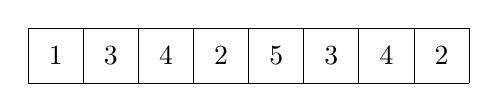
\begin{tikzpicture}[scale=0.7]
\draw (0,0) grid (8,1);

\node at (0.5,0.5) {$1$};
\node at (1.5,0.5) {$3$};
\node at (2.5,0.5) {$4$};
\node at (3.5,0.5) {$2$};
\node at (4.5,0.5) {$5$};
\node at (5.5,0.5) {$3$};
\node at (6.5,0.5) {$4$};
\node at (7.5,0.5) {$2$};
\end{tikzpicture}
\end{center}

First, the elements 1, 3 and 4 are added to the stack,
because each element is larger than the previous element.
Thus, the nearest smaller element of 4 is 3,
and the nearest smaller element of 3 is 1.
\begin{center}
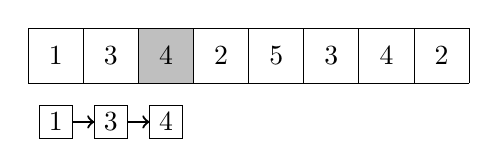
\begin{tikzpicture}[scale=0.7]
\fill[color=lightgray] (2,0) rectangle (3,1);
\draw (0,0) grid (8,1);

\node at (0.5,0.5) {$1$};
\node at (1.5,0.5) {$3$};
\node at (2.5,0.5) {$4$};
\node at (3.5,0.5) {$2$};
\node at (4.5,0.5) {$5$};
\node at (5.5,0.5) {$3$};
\node at (6.5,0.5) {$4$};
\node at (7.5,0.5) {$2$};

\draw (0.2,0.2-1.2) rectangle (0.8,0.8-1.2);
\draw (1.2,0.2-1.2) rectangle (1.8,0.8-1.2);
\draw (2.2,0.2-1.2) rectangle (2.8,0.8-1.2);

\node at (0.5,0.5-1.2) {$1$};
\node at (1.5,0.5-1.2) {$3$};
\node at (2.5,0.5-1.2) {$4$};

\draw[->,thick] (0.8,0.5-1.2) -- (1.2,0.5-1.2);
\draw[->,thick] (1.8,0.5-1.2) -- (2.2,0.5-1.2);
\end{tikzpicture}
\end{center}

The next element 2 is smaller than the two top
elements in the stack.
Thus, the elements 3 and 4 are removed from the stack,
and then the element 2 is added to the stack.
Its nearest smaller element is 1:
\begin{center}
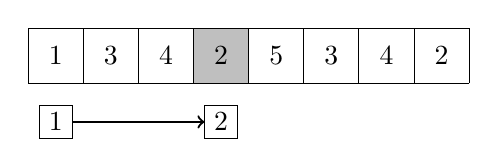
\begin{tikzpicture}[scale=0.7]
\fill[color=lightgray] (3,0) rectangle (4,1);
\draw (0,0) grid (8,1);

\node at (0.5,0.5) {$1$};
\node at (1.5,0.5) {$3$};
\node at (2.5,0.5) {$4$};
\node at (3.5,0.5) {$2$};
\node at (4.5,0.5) {$5$};
\node at (5.5,0.5) {$3$};
\node at (6.5,0.5) {$4$};
\node at (7.5,0.5) {$2$};

\draw (0.2,0.2-1.2) rectangle (0.8,0.8-1.2);
\draw (3.2,0.2-1.2) rectangle (3.8,0.8-1.2);

\node at (0.5,0.5-1.2) {$1$};
\node at (3.5,0.5-1.2) {$2$};

\draw[->,thick] (0.8,0.5-1.2) -- (3.2,0.5-1.2);
\end{tikzpicture}
\end{center}

Then, the element 5 is larger than the element 2,
so it will be added to the stack, and
its nearest smaller element is 2:
\begin{center}
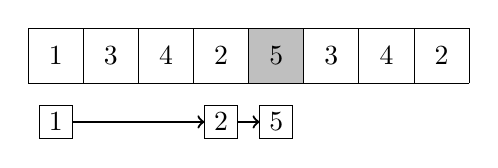
\begin{tikzpicture}[scale=0.7]
\fill[color=lightgray] (4,0) rectangle (5,1);
\draw (0,0) grid (8,1);

\node at (0.5,0.5) {$1$};
\node at (1.5,0.5) {$3$};
\node at (2.5,0.5) {$4$};
\node at (3.5,0.5) {$2$};
\node at (4.5,0.5) {$5$};
\node at (5.5,0.5) {$3$};
\node at (6.5,0.5) {$4$};
\node at (7.5,0.5) {$2$};

\draw (0.2,0.2-1.2) rectangle (0.8,0.8-1.2);
\draw (3.2,0.2-1.2) rectangle (3.8,0.8-1.2);
\draw (4.2,0.2-1.2) rectangle (4.8,0.8-1.2);

\node at (0.5,0.5-1.2) {$1$};
\node at (3.5,0.5-1.2) {$2$};
\node at (4.5,0.5-1.2) {$5$};

\draw[->,thick] (0.8,0.5-1.2) -- (3.2,0.5-1.2);
\draw[->,thick] (3.8,0.5-1.2) -- (4.2,0.5-1.2);
\end{tikzpicture}
\end{center}

After this, the element 5 is removed from the stack
and the elements 3 and 4 are added to the stack:
\begin{center}
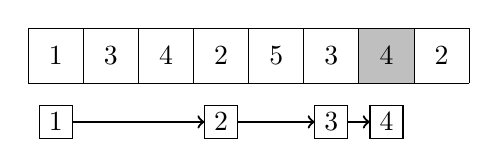
\begin{tikzpicture}[scale=0.7]
\fill[color=lightgray] (6,0) rectangle (7,1);
\draw (0,0) grid (8,1);

\node at (0.5,0.5) {$1$};
\node at (1.5,0.5) {$3$};
\node at (2.5,0.5) {$4$};
\node at (3.5,0.5) {$2$};
\node at (4.5,0.5) {$5$};
\node at (5.5,0.5) {$3$};
\node at (6.5,0.5) {$4$};
\node at (7.5,0.5) {$2$};

\draw (0.2,0.2-1.2) rectangle (0.8,0.8-1.2);
\draw (3.2,0.2-1.2) rectangle (3.8,0.8-1.2);
\draw (5.2,0.2-1.2) rectangle (5.8,0.8-1.2);
\draw (6.2,0.2-1.2) rectangle (6.8,0.8-1.2);

\node at (0.5,0.5-1.2) {$1$};
\node at (3.5,0.5-1.2) {$2$};
\node at (5.5,0.5-1.2) {$3$};
\node at (6.5,0.5-1.2) {$4$};

\draw[->,thick] (0.8,0.5-1.2) -- (3.2,0.5-1.2);
\draw[->,thick] (3.8,0.5-1.2) -- (5.2,0.5-1.2);
\draw[->,thick] (5.8,0.5-1.2) -- (6.2,0.5-1.2);
\end{tikzpicture}
\end{center}

Finally, all elements except 1 are removed
from the stack and the last element 2
is added to the stack:

\begin{center}
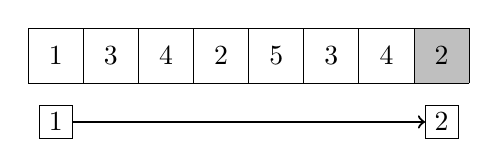
\begin{tikzpicture}[scale=0.7]
\fill[color=lightgray] (7,0) rectangle (8,1);
\draw (0,0) grid (8,1);

\node at (0.5,0.5) {$1$};
\node at (1.5,0.5) {$3$};
\node at (2.5,0.5) {$4$};
\node at (3.5,0.5) {$2$};
\node at (4.5,0.5) {$5$};
\node at (5.5,0.5) {$3$};
\node at (6.5,0.5) {$4$};
\node at (7.5,0.5) {$2$};

\draw (0.2,0.2-1.2) rectangle (0.8,0.8-1.2);
\draw (7.2,0.2-1.2) rectangle (7.8,0.8-1.2);

\node at (0.5,0.5-1.2) {$1$};
\node at (7.5,0.5-1.2) {$2$};

\draw[->,thick] (0.8,0.5-1.2) -- (7.2,0.5-1.2);
\end{tikzpicture}
\end{center}

The efficiency of the algorithm depends on
the total number of stack operations.
If the current element is larger than
the top element in the stack, it is directly
added to the stack, which is efficient.
However, sometimes the stack can contain several
larger elements and it takes time to remove them.
Still, each element is added \emph{exactly once} to the stack
and removed \emph{at most once} from the stack.
Thus, each element causes $O(1)$ stack operations,
and the algorithm works in $O(n)$ time.

\section{Sliding window minimum}

\index{sliding window}
\index{sliding window minimum}

A \key{sliding window} is a constant-size subarray
that moves from left to right through the array.
At each window position,
we want to calculate some information
about the elements inside the window.
In this section, we focus on the problem
of maintaining the \key{sliding window minimum},
which means that
we should report the smallest value inside each window.

The sliding window minimum can be calculated
using a similar idea that we used to calculate
the nearest smaller elements.
We maintain a queue
where each element is larger than
the previous element,
and the first element
always corresponds to the minimum element inside the window.
After each window move,
we remove elements from the end of the queue
until the last queue element
is smaller than the new window element,
or the queue becomes empty.
We also remove the first queue element
if it is not inside the window anymore.
Finally, we add the new window element
to the end of the queue.

As an example, consider the following array:

\begin{center}
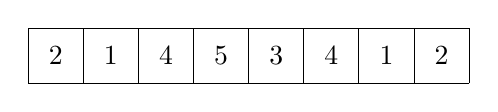
\begin{tikzpicture}[scale=0.7]
\draw (0,0) grid (8,1);

\node at (0.5,0.5) {$2$};
\node at (1.5,0.5) {$1$};
\node at (2.5,0.5) {$4$};
\node at (3.5,0.5) {$5$};
\node at (4.5,0.5) {$3$};
\node at (5.5,0.5) {$4$};
\node at (6.5,0.5) {$1$};
\node at (7.5,0.5) {$2$};
\end{tikzpicture}
\end{center}

Suppose that the size of the sliding window is 4.
At the first window position, the smallest value is 1:
\begin{center}
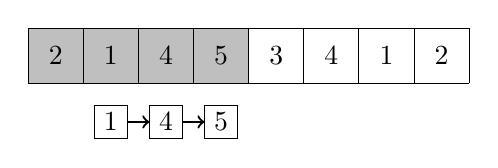
\begin{tikzpicture}[scale=0.7]
\fill[color=lightgray] (0,0) rectangle (4,1);
\draw (0,0) grid (8,1);

\node at (0.5,0.5) {$2$};
\node at (1.5,0.5) {$1$};
\node at (2.5,0.5) {$4$};
\node at (3.5,0.5) {$5$};
\node at (4.5,0.5) {$3$};
\node at (5.5,0.5) {$4$};
\node at (6.5,0.5) {$1$};
\node at (7.5,0.5) {$2$};

\draw (1.2,0.2-1.2) rectangle (1.8,0.8-1.2);
\draw (2.2,0.2-1.2) rectangle (2.8,0.8-1.2);
\draw (3.2,0.2-1.2) rectangle (3.8,0.8-1.2);

\node at (1.5,0.5-1.2) {$1$};
\node at (2.5,0.5-1.2) {$4$};
\node at (3.5,0.5-1.2) {$5$};

\draw[->,thick] (1.8,0.5-1.2) -- (2.2,0.5-1.2);
\draw[->,thick] (2.8,0.5-1.2) -- (3.2,0.5-1.2);
\end{tikzpicture}
\end{center}

Then the window moves one step right.
The new element 3 is smaller than the elements
4 and 5 in the queue, so the elements 4 and 5
are removed from the queue
and the element 3 is added to the queue.
The smallest value is still 1.
\begin{center}
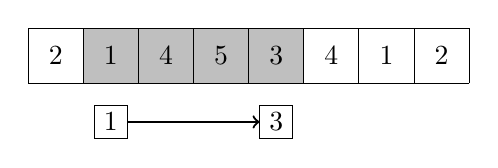
\begin{tikzpicture}[scale=0.7]
\fill[color=lightgray] (1,0) rectangle (5,1);
\draw (0,0) grid (8,1);

\node at (0.5,0.5) {$2$};
\node at (1.5,0.5) {$1$};
\node at (2.5,0.5) {$4$};
\node at (3.5,0.5) {$5$};
\node at (4.5,0.5) {$3$};
\node at (5.5,0.5) {$4$};
\node at (6.5,0.5) {$1$};
\node at (7.5,0.5) {$2$};

\draw (1.2,0.2-1.2) rectangle (1.8,0.8-1.2);
\draw (4.2,0.2-1.2) rectangle (4.8,0.8-1.2);

\node at (1.5,0.5-1.2) {$1$};
\node at (4.5,0.5-1.2) {$3$};

\draw[->,thick] (1.8,0.5-1.2) -- (4.2,0.5-1.2);
\end{tikzpicture}
\end{center}

After this, the window moves again,
and the smallest element 1
does not belong to the window anymore.
Thus, it is removed from the queue and the smallest
value is now 3. Also the new element 4
is added to the queue.
\begin{center}
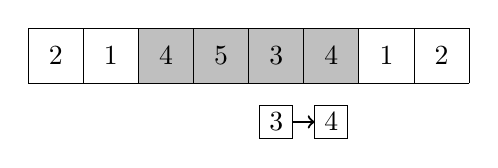
\begin{tikzpicture}[scale=0.7]
\fill[color=lightgray] (2,0) rectangle (6,1);
\draw (0,0) grid (8,1);

\node at (0.5,0.5) {$2$};
\node at (1.5,0.5) {$1$};
\node at (2.5,0.5) {$4$};
\node at (3.5,0.5) {$5$};
\node at (4.5,0.5) {$3$};
\node at (5.5,0.5) {$4$};
\node at (6.5,0.5) {$1$};
\node at (7.5,0.5) {$2$};

\draw (4.2,0.2-1.2) rectangle (4.8,0.8-1.2);
\draw (5.2,0.2-1.2) rectangle (5.8,0.8-1.2);

\node at (4.5,0.5-1.2) {$3$};
\node at (5.5,0.5-1.2) {$4$};

\draw[->,thick] (4.8,0.5-1.2) -- (5.2,0.5-1.2);
\end{tikzpicture}
\end{center}

The next new element 1 is smaller than all elements
in the queue.
Thus, all elements are removed from the queue
and it will only contain the element 1:
\begin{center}
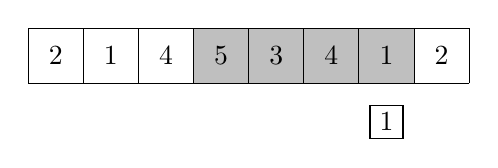
\begin{tikzpicture}[scale=0.7]
\fill[color=lightgray] (3,0) rectangle (7,1);
\draw (0,0) grid (8,1);

\node at (0.5,0.5) {$2$};
\node at (1.5,0.5) {$1$};
\node at (2.5,0.5) {$4$};
\node at (3.5,0.5) {$5$};
\node at (4.5,0.5) {$3$};
\node at (5.5,0.5) {$4$};
\node at (6.5,0.5) {$1$};
\node at (7.5,0.5) {$2$};

\draw (6.2,0.2-1.2) rectangle (6.8,0.8-1.2);

\node at (6.5,0.5-1.2) {$1$};
\end{tikzpicture}
\end{center}

Finally the window reaches its last position.
The element 2 is added to the queue,
but the smallest value inside the window
is still 1.
\begin{center}
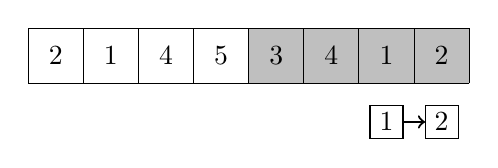
\begin{tikzpicture}[scale=0.7]
\fill[color=lightgray] (4,0) rectangle (8,1);
\draw (0,0) grid (8,1);

\node at (0.5,0.5) {$2$};
\node at (1.5,0.5) {$1$};
\node at (2.5,0.5) {$4$};
\node at (3.5,0.5) {$5$};
\node at (4.5,0.5) {$3$};
\node at (5.5,0.5) {$4$};
\node at (6.5,0.5) {$1$};
\node at (7.5,0.5) {$2$};

\draw (6.2,0.2-1.2) rectangle (6.8,0.8-1.2);
\draw (7.2,0.2-1.2) rectangle (7.8,0.8-1.2);

\node at (6.5,0.5-1.2) {$1$};
\node at (7.5,0.5-1.2) {$2$};

\draw[->,thick] (6.8,0.5-1.2) -- (7.2,0.5-1.2);
\end{tikzpicture}
\end{center}

Since each array element
is added to the queue exactly once and
removed from the queue at most once,
the algorithm works in $O(n)$ time.
